\subsection{Circuito III: VFA-CFA}

\hspace{1mm} Se diseña una red de compensación cero-polo, con el propósito de cancelar el polo ubicado en \(5.06~MHz\) del amplificador VFA y lograr tener en la frecuencia \(f_g= 2Mhz\). La configuración de esta red se presenta en la siguiente figura:

\begin{figure}[!h]
    \centering
    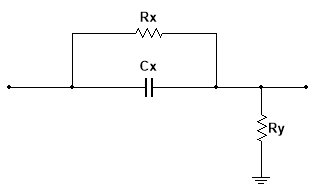
\includegraphics[width=0.5\linewidth]{Imagenes/Red de compensacion RC.png}
    \caption{Red de Compensación RC.}
\end{figure}

\hspace{1mm} Se aplica esta red de compensación (cero - polo) para compensar el efecto del polo existente en la frecuencia de \(5.06~MHz\).

\bigskip
\hspace{1mm} La función de transferencia de la red que se aplica es la siguiente:

\begin{equation}
    A_c(s) = \frac{R_y}{R_x + R_y} \cdot \frac{1 + sC_x R_x}{1 + sC_x (R_x // R_y)}
\end{equation}

\hspace{1mm} Donde se han definido las siguientes notaciones:

\begin{itemize}[itemsep=1pt]
    \item \(k_{comp}=\frac{R_y}{R_x + R_y}\)
    \item \( \omega_{pcomp} =  \frac{1 }{1 + sC_x (R_x // R_y)}\)
    \item \(\omega_{zcomp} = \frac{1 }{ C_xR_x}\)
\end{itemize}

\hspace{1mm} Como el cero del compensador debe cancelar el polo de frecuencia más alta del VFA, entonces:
\begin{equation}
    \omega_{zcomp} = \omega_2 = 2\pi \cdot 5.06~Mrps
\end{equation}
\hspace{1mm} El polo de compensación se encuentra una octava por encima de este cero para mantener la relación de ganancia especificada en el marco teórico. Entonces:

\begin{equation}
    \omega _{pcomp} = 2\omega _{zcomp} = 2\pi \cdot 10.12~Mrps
\end{equation}

\hspace{1mm} A partir de estos valores se pudo calcular la ganancia del compensador \(k_{comp}\)

\begin{equation}
    k_{comp} = \frac{\omega_{zcomp}}{\omega _{pcomp}} = \frac{2\pi \cdot 5.06~Mrps}{2\pi \cdot 10.12~Mrps}
    \end{equation}
\begin{equation}
    \boxed{
    k_{comp} = 0.5
    }
\end{equation}
\hspace{1mm} Por lo tanto, \(k_{comp}\) es.

\begin{equation}
    k_{comp} = \frac{R_y}{R_x + R_y} = 0.5
\end{equation}

\hspace{1mm} Se obetiene la relación entre las resistencias.

\begin{equation}
    \frac{R_y}{R_x + R_y} = \frac{1}{2} \Longrightarrow 2R_y = R_x + R_y \Longrightarrow 2 = \frac{R_x}{R_y} + 1
\end{equation}

\begin{equation}
    \boxed{
    1 = \frac{R_x}{R_y}
    }
\end{equation}

\hspace{1mm} Entonces, se consideran los siguientes valores:

\begin{equation}
    \boxed{
    R_x = R_y = 1~k\Omega
    }
\end{equation}

\hspace{1mm} Con dichos valores se puede calcular el capacitor \(C_x\) despejando la fórmula de \(\omega_{zcomp}\).

\begin{equation}
    \omega_{zcomp} = \frac{1}{C_x R_x} = 2\pi \cdot 5.06~Mrps
\end{equation}

\begin{equation}
    C_x = \frac{1}{2\pi \cdot 5.06~Mrps \cdot 1~k\Omega}
\end{equation}

\begin{equation}
    \boxed{
    C_x = 31~pF
    }
\end{equation}

\hspace{1mm} Se agrega el compensador y se obtiene la siguiente función de transferencia del lazo de realimentación: ---------

\begin{equation}
    T(s) = -A_d(s) \cdot A_c(s) \cdot A_{vf2} (s) = - \frac{kA_d(0)}{\left(1+\frac{s}{\omega_1}\right)\left(1+\frac{s}{\omega_2}\right)} \cdot k_{comp} \frac{\left(1 + \frac{s}{\omega_{zcomp}}\right)}{\left(1+\frac{s}{\omega_{pcomp}}\right)} \cdot A_{vf2}(s)
\end{equation}

\hspace{1mm} Donde:

\begin{itemize}[itemsep=1pt]
    \item k es la realimentación del VFA.
    \item \(A_d(0)\) la ganancia del VFA.
    \item \(A_{vf2}\) la función de transferencia del CFA.
    \item \( \omega_1 \) y \( \omega_2 \) los polos del VFA.
\end{itemize}

\hspace{1mm} Se observa que el valor de \(k_{comp}\) produce atenuación a la ganancia del sistema. Se ajusta la ganancia a lazo cerrado del CFA, teniendo en cuenta que \( k_{comp} = 0.5 \):

\begin{equation}
    A_{vf2 comp} (s) = 2A_{vf2}(s)
\end{equation}

\hspace{1mm} Esta relación garantiza que la atenuación provocada por \(k_{comp}\) se compense adecuadamente en la ganancia a lazo cerrado.

\hspace{1mm} Como \(A_{vf2}\) es:

\begin{equation}
    A_{vf2} = 1 + \frac{R_2}{R_1}
\end{equation}

\hspace{1mm} Se reemplaza:

\begin{equation}
    A_{vf2 comp} (s) = 2 \left( 1 + \frac{R_2}{R_1} \right) = 2 \cdot 20
\end{equation}

\begin{equation}
    \boxed{
    A_{vf2 comp} (s) = 40
    }
\end{equation}

\hspace{1mm} El polo del amplificador operacional LM6181 (CFA) permanece invariable con respecto al caso anterior. El valor de \(R_2\) continúa siendo \(850~\Omega\). Se calcula \(R_1\) como:

\begin{equation}
    \frac{R_2}{R_1} = 40 - 1 \Longrightarrow R_1 = \frac{850~\Omega}{39}
\end{equation}

\begin{equation}
    \boxed{
    R_1 = 21.8~\Omega
    }
\end{equation}

\hspace{1mm} El margen de fase ( \(M\varphi\) ) se determina como la diferencia entre \(180^o\) y la suma de los ángulos de las funciones de ganancia a lazo cerrado del Amplificador (VFA1), la función de ganancia a lazo cerrado del Compensador de Fase Avanzada (CFA), y el ángulo de la función de transferencia del Compensador. En este caso:

\begin{equation}
    M\varphi = 180^o - arctg \left(  \frac{f_g}{f_{VFA1}}\right) - arctg \left( \frac{f_g}{f_{comp}} \right) - arctg \left( \frac{f_g}{f_{CFA}} \right)
\end{equation}

\begin{equation}
   M\varphi = 180^o - 90^o - 11.12^o - 2.93^o
\end{equation}

\begin{equation}
    \boxed{
    M\varphi = 75.9^o
    }
\end{equation}
-----------------------------------------------------------

\hspace{1mm} El ancho de banda potencial permanece inalterado en relación con el caso anterior, manteniéndose en \(2~MHz\). La frecuencia del polo de la función de transferencia a lazo cerrado se calcula aplicando el producto ganancia por ancho de banda:

\begin{equation}
    A_{vf} (0) \cdot f_g = A_{vf}(-3~dB) \cdot f_p
\end{equation}

\newpage
\hspace{1mm} Se despejó \(f_p\)

\begin{equation}
    f_p = \frac{A_{vf} (0) \cdot f_g}{A_{vf}(-3~dB)} = \frac{10.2~MHz}{7.079}
\end{equation}

\begin{equation}
    \boxed{
    f_p = 2.825~MHz
    }
\end{equation}

\hspace{1mm} Por lo tanto, el ancho de banda a \(-3~dB\) resulta igual a la frecuencia del polo, es decir, \(2.825~MHz\).

\subsubsection{Simulación}

\hspace{1mm} Se obtuvo así el circuito completo con red de compensación el cual se realizó con el simulador Multisim V.14.0.

\begin{figure}[!h]
    \centering
    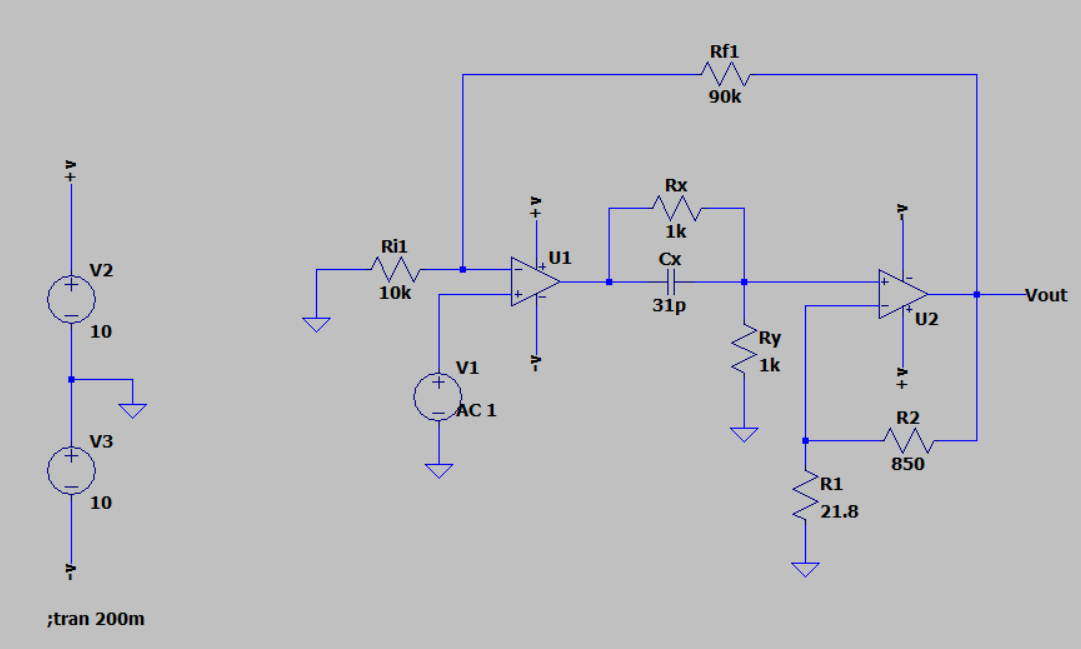
\includegraphics[width=0.7\linewidth]{VFA CFA Compensado/Imágenes/Circuito 3.png}
    \caption{Circuito Completo con Compensador.}
\end{figure}

\hspace{1mm} En el cual, como en el caso anterior, se insertó una señal sinusoidal con un valor de tensión pico de \(10~mV\) con una frecuencia de \( 1~kHz \) se obtuvieron las siguientes gráficas a la entrada (color rojo) y a la salida (color azul).

\begin{figure}[!h]
    \centering
    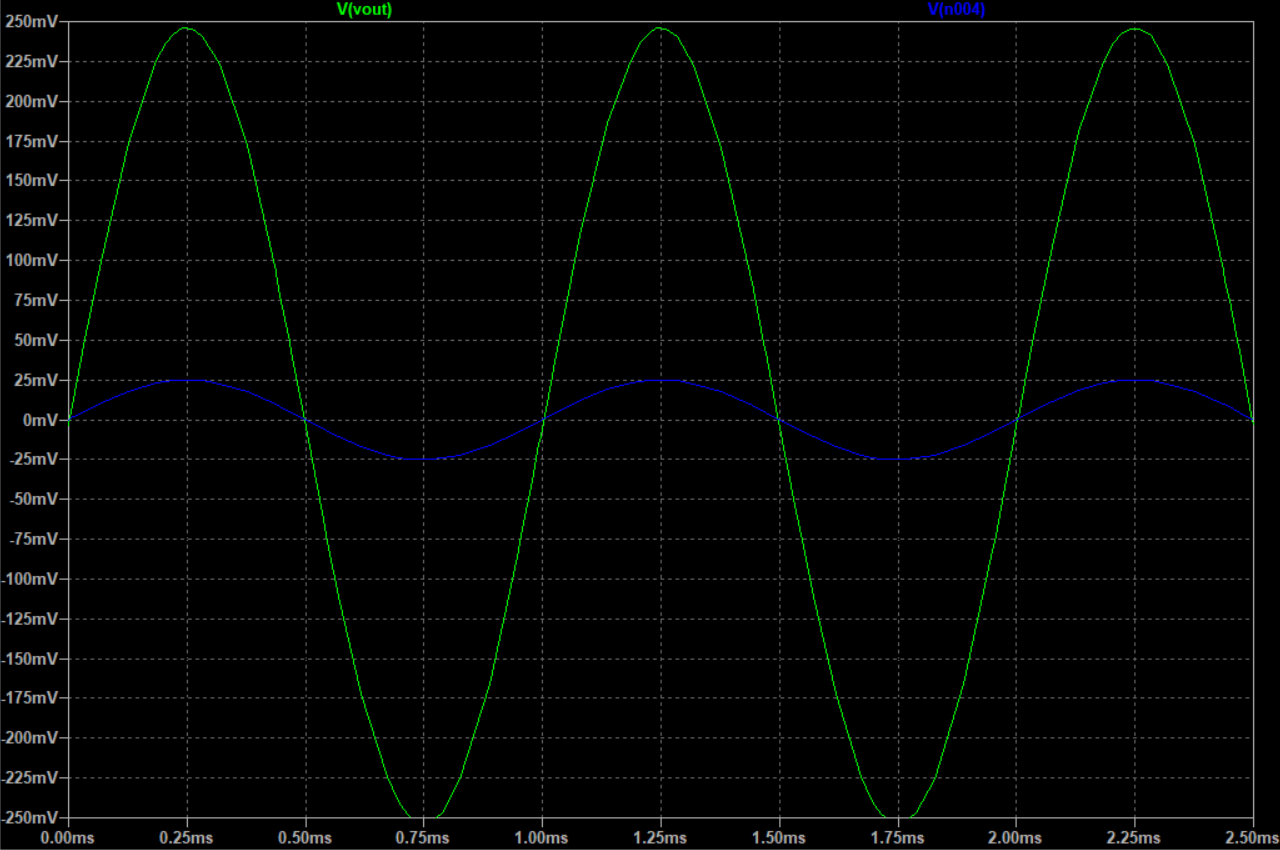
\includegraphics[width=0.7\linewidth]{VFA CFA Compensado/Imágenes/Circuito 3 - Simulacion.png}
    \caption{Ganancia del circuito compensado.}
\end{figure}

\hspace{1mm} En donde se puede comprobar que para un valor de entrada de \( 25~mV \) se obtiene a la salida \( 250mV~mV \). Se calcula la ganancia con los valores medidos

\begin{equation}
    G = \frac{250~mV}{25~mV}
\end{equation}

\begin{equation}
    \boxed{
    G = 10
    }
\end{equation}

\newpage
.\hspace{1mm} Se genera el diagrama de Bode del circuito propuestos. En este diagrama, se observa una ganancia de \(20~dB\) y una caída de \(-3~dB\), la cual se produce a una frecuencia de \(2~MHz\).

\begin{figure}[!h]
    \centering
    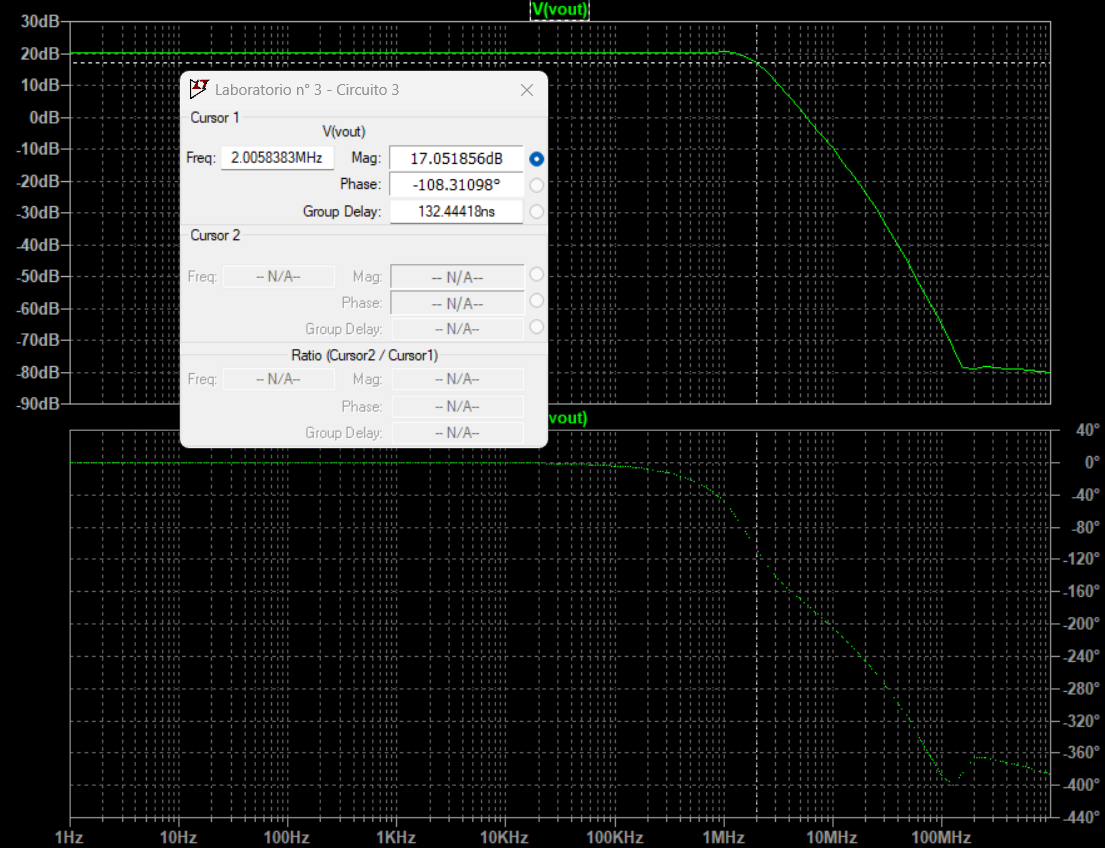
\includegraphics[width=0.7\linewidth]{VFA CFA Compensado/Imágenes/Circuito 3 - Bode.png}
\end{figure}